% ============================================
% AEGIS Entropy --- Final Report
% Adaptive Entropy-based Gateway for Intrusion Suppression
% ============================================
\documentclass[12pt,a4paper]{report}

% --- Encoding & Language ---
\usepackage[utf8]{inputenc}
\usepackage[T1]{fontenc}
\usepackage[english]{babel}
\usepackage{lmodern}

% --- Page Layout ---
\usepackage[left=2.5cm,right=2.5cm,top=2.5cm,bottom=2.5cm]{geometry}
\setlength{\parindent}{0pt}
\setlength{\parskip}{0.65em}
\renewcommand{\arraystretch}{1.25}

% --- Math ---
\usepackage{amsmath,amssymb}

% --- Graphics ---
\usepackage{graphicx}
\graphicspath{
    {figures/data/}
    {figures/capture/}
    {figures/defense/}
}
\usepackage{float}
\usepackage{caption}
\usepackage{subcaption}

% --- Tables ---
\usepackage{array}
\usepackage{longtable}
\usepackage{booktabs}
\usepackage{tabularx}
\usepackage[table]{xcolor}

% --- Lists ---
\usepackage{enumitem}
\setlist[itemize]{topsep=0.2em,itemsep=0.2em}
\setlist[enumerate]{topsep=0.2em,itemsep=0.25em}

% --- Code Listings ---
\usepackage{listings}
\lstdefinestyle{pythonstyle}{
    language=Python,
    basicstyle=\ttfamily\small,
    keywordstyle=\color{blue}\bfseries,
    stringstyle=\color{red},
    commentstyle=\color{gray}\itshape,
    numbers=left,
    numberstyle=\tiny\color{gray},
    stepnumber=1,
    numbersep=5pt,
    backgroundcolor=\color{gray!5},
    frame=single,
    rulecolor=\color{gray!30},
    breaklines=true,
    showstringspaces=false,
    tabsize=4,
    captionpos=b
}
\lstset{style=pythonstyle}

% --- TikZ ---
\usepackage{tikz}
\usetikzlibrary{shapes.geometric, arrows.meta, positioning, calc, decorations.pathmorphing, fit, backgrounds}
\usepackage{pgfplots}
\pgfplotsset{compat=1.18}

% --- Colors for diagrams ---
\definecolor{darkbg}{HTML}{0b0f19}
\definecolor{cyan}{HTML}{22d3ee}
\definecolor{green}{HTML}{34d399}
\definecolor{red}{HTML}{f87171}
\definecolor{amber}{HTML}{fbbf24}
\definecolor{purple}{HTML}{a78bfa}
\definecolor{codebg}{HTML}{1a2332}
\definecolor{codegray}{HTML}{94a3b8}
\definecolor{LightGray}{HTML}{F2F2F2}
\definecolor{LightBlue}{HTML}{D9EAF7}

% --- Hyperlinks ---
\usepackage{hyperref}
\hypersetup{
    colorlinks=true,
    linkcolor=blue!70!black,
    urlcolor=blue!60!black,
    citecolor=blue!70!black,
    pdftitle={AEGIS Entropy --- Final Report},
    pdfauthor={AEGIS Entropy Team}
}

% --- Headers & Footers ---
\usepackage{fancyhdr}
\pagestyle{fancy}
\fancyhf{}
\fancyhead[L]{\small\textsc{AEGIS Entropy}}
\fancyhead[R]{\small\textsc{Final Report}}
\fancyfoot[C]{\thepage}
\renewcommand{\headrulewidth}{0.4pt}

% --- Chapter/Section Formatting ---
\usepackage{titlesec}
\titleformat{\chapter}[display]
    {\normalfont\Large\bfseries\color{blue!80!black}}
    {\chaptertitlename\ \thechapter}
    {0.5em}
    {}
\titleformat{\section}{\normalfont\large\bfseries\color{blue!70!black}}{\thesection}{1em}{}
\titleformat{\subsection}{\normalfont\normalsize\bfseries\color{blue!60!black}}{\thesubsection}{1em}{}

% --- Custom Commands ---
\newcolumntype{Y}{>{\raggedright\arraybackslash}X}
\newcolumntype{L}[1]{>{\raggedright\arraybackslash}p{#1}}
\newcommand{\code}[1]{\texttt{\detokenize{#1}}}

% --- Placeholder Command ---
\newcommand{\todo}[1]{\textcolor{red}{\textbf{[TODO: #1]}}}
\newcommand{\tobewritten}[1]{\textcolor{orange}{\textit{[To be written by #1]}}}

% ============================================
\begin{document}

% --- Title Page ---
\begin{titlepage}
\centering
\vspace*{1cm}

{\Large\textsc{ENSA Kenitra}}\\[0.2cm]
{\small\textsc{Networks and Telecommunication Systems Engineering}}\\[0.2cm]
{\small\textsc{AI Module --- Semester 2 --- 2026}}

\vspace{2cm}

\rule{\textwidth}{0.5pt}\\[0.8cm]

{\Huge\bfseries AEGIS}\\[0.4cm]
{\Large Adaptive Entropy-based Gateway\\for Intrusion Suppression}\\[0.3cm]
{\large\bfseries Final Report --- Port Scan Detection and Response}

\vspace{0.8cm}
\rule{\textwidth}{0.5pt}

\vspace{2cm}

\begin{minipage}{0.85\textwidth}
\centering
\begin{tabular}{rl}
\textbf{Team:} & Adil Lekhbioui (ML, Dashboard, Response, Integration)\\
 & Khadija Nafia (ML, Preprocessing, Training)\\
 & El Yazid (Deception, MTD, Honeypot)\\
 & Moulay Anas (Capture, Network Lab)\\
 & El Kartouti Anas (Conception, Documentation)\\[0.5cm]
\textbf{Supervisor:} & Prof. Aniss Moumen\\[0.5cm]
\textbf{Date:} & June 2026\\
\end{tabular}
\end{minipage}

\vfill

{\small ENSA Kenitra --- Morocco}
\end{titlepage}

% --- Abstract ---
\newpage
\section*{Abstract}
\addcontentsline{toc}{section}{Abstract}

This report presents the design, implementation, and evaluation of AEGIS Entropy, an AI-based network intrusion detection and prevention system for port scan attacks. The system combines supervised classifiers (Random Forest, XGBoost) with an unsupervised anomaly detector (Isolation Forest) to identify reconnaissance activity from network flow features. A Moving Target Defense layer actively reshapes the attack surface through port rotation, honeypot deployment, and automated IP blocking. The system operates in offline mode for batch analysis of Nmap scans and live mode for real-time detection on a controlled LAN. On the CICIDS2017 dataset, the detection pipeline achieves 99.91\% accuracy with a 0.11\% false positive rate, exceeding all project success criteria. The defense subsystem achieves full-stack activation in under 520ms.

\vspace{1em}
\noindent\textbf{Keywords:} Network Intrusion Detection, Port Scan, Machine Learning, Random Forest, XGBoost, Moving Target Defense, Honeypot

% --- Table of Contents ---
\tableofcontents
\listoffigures
\listoftables
\newpage

% ============================================
% CHAPTER 1: General Introduction
% ============================================
\input{chapters/ch01_introduction}

% ============================================
% CHAPTER 2: State of the Art
% ============================================
\input{chapters/ch02_state_of_art}

% ============================================
% CHAPTER 3: Understanding the Problem and the Data
% ============================================
\input{chapters/ch03_understanding}

% ============================================
% CHAPTER 4: Data Exploration and Preparation
% ============================================
% ============================================
% Chapter 4: Data Exploration and Preparation
% ============================================
% Rewritten — June 2026
% Based on Khadija's ML pipeline work, retrained models

\chapter{Data Exploration and Preparation}

\section{Introduction}

Before any machine learning model can be trained, the data must be understood, cleaned, and properly prepared. This chapter walks through the complete data preparation pipeline that transforms raw network flow records from the CICIDS2017 dataset into a clean, balanced, and standardized dataset ready for model training. Every decision made at this stage --- how to handle missing values, what to do with outliers, whether to balance the classes --- directly impacts the quality of the detection system. For this reason, we follow the PDCA (\textit{Plan-Do-Check-Act}) methodology, documenting not only what was done but why each choice was made.

The primary objective is to produce a dataset that enables the detection pipeline to meet the success criteria defined in the project plan:
\begin{itemize}
    \item \textbf{F1-Score} $\geq$ 88\%
    \item \textbf{Accuracy} $\geq$ 90\%
    \item \textbf{False Positive Rate (FPR)} $<$ 6\%
\end{itemize}

\section{Dataset Overview}

\subsection{What is CICIDS2017?}

The \textbf{CICIDS2017} dataset (\textit{Canadian Institute for Cybersecurity Intrusion Detection System}, 2017) is one of the most widely cited academic benchmarks for network intrusion detection research. Unlike older datasets such as KDD-99 --- which dates back to 1999 and no longer reflects modern network behavior --- CICIDS2017 was generated in a controlled environment that replicates realistic network traffic conditions, including both benign user activity and simulated attacks across multiple days.

\begin{table}[H]
\centering
\caption{Dataset characteristics — CICIDS2017 PortScan subset}
\label{tab:dataset}
\begin{tabular}{ll}
\toprule
\textbf{Property} & \textbf{Value} \\
\midrule
Number of flow records (rows) & 286,467 \\
Number of raw features (columns) & 79 \\
\texttt{PortScan} class & 158,930 (55.48\%) \\
\texttt{BENIGN} class & 127,537 (44.52\%) \\
File used & \texttt{Friday-WorkingHours-Afternoon-PortScan.pcap\_ISCX.csv} \\
Format & CSV — aggregated network flows (\textit{flow-level}) \\
\bottomrule
\end{tabular}
\end{table}

\subsection{Understanding the Class Distribution}

The dataset contains 55.48\% PortScan traffic and 44.52\% benign traffic. This is a slight imbalance in favor of the attack class, which is unusual: in most intrusion detection datasets, attacks represent a small minority (typically $<$ 5\%). Here, the PortScan class actually constitutes the \textit{majority}. This has important consequences:

\begin{itemize}
    \item \textbf{For supervised models} (Random Forest, XGBoost): the imbalance is moderate and can be managed with SMOTE (Section~\ref{sec:smote}).
    \item \textbf{For unsupervised models} (Isolation Forest): the majority class being the attack class creates a fundamental problem, which we analyse in detail in Chapter~5 (\textit{majority anomaly paradox}).
\end{itemize}

\begin{figure}[H]
\centering

\includegraphics[width=0.65\textwidth]{class_distribution.png}
\caption{Class distribution in the CICIDS2017 PortScan dataset. The attack class (PortScan) constitutes 55.48\% of the total records --- a slight majority.}
\label{fig:class_dist}
\end{figure}

\section{Feature Selection}

\subsection{From the Data Dictionary to the CSV}

The project's Data Dictionary defines 13 features theoretically relevant for detecting port scan attacks. However, CICIDS2017 is a collection of aggregated network flows (\textit{flow-level data}), not raw packet captures. As a result, not all 13 features are available from the CSV. A mapping process was conducted to find the best proxy for each theoretical feature.

\begin{longtable}{p{3.5cm}cp{3.5cm}p{4.5cm}}
\caption{Feature mapping: Data Dictionary $\rightarrow$ CICIDS2017 CSV columns} \\
\label{tab:feature_mapping} \\
\toprule
\textbf{Feature (Dictionary)} & \textbf{Avail.} & \textbf{CSV Column} & \textbf{Justification} \\
\midrule
\endfirsthead
\toprule
\textbf{Feature (Dictionary)} & \textbf{Avail.} & \textbf{CSV Column} & \textbf{Justification} \\
\midrule
\endhead
Distinct Dst Ports & $\approx$ & Destination Port & Proxy: scanners target many different ports, so the port number itself carries discriminative signal \\
SYN Flag Count & \checkmark & SYN Flag Count & Direct match — counts SYN packets per flow \\
RST Flag Count & \checkmark & RST Flag Count & Direct match — counts RST (reset) packets per flow \\
Flow Duration & \checkmark & Flow Duration & Direct match — scan flows are typically very short \\
Total Fwd Packets & \checkmark & Total Fwd Packets & Direct match — scanners send few packets per probe \\
ACK Flag Count & \checkmark & ACK Flag Count & Direct match — counts ACK packets per flow \\
IAT Mean & \checkmark & Flow IAT Mean & Direct match — inter-arrival time between packets \\
Bwd Packet Length & \checkmark & Bwd Packet Length Mean & Mean variant — average backward packet size \\
TCP Window Size & \checkmark & Init\_Win\_bytes\_forward & Best proxy — initial window size in the forward direction \\
\midrule
Unique Dst IPs & $\times$ & --- & Absent from CSV; available only in live capture mode \\
TTL Value & $\times$ & --- & Absent from flow-level data; packet-level feature \\
Shadow Node Interaction & N/A & Placeholder = 0 & Reserved for future integration with the honeypot module \\
MTD Port Delta & N/A & Placeholder = 0 & Reserved for future integration with the MTD module \\
\bottomrule
\end{longtable}

\subsection{Final Feature Set: 11 Features}

The pipeline uses \textbf{11 features}: 9 extracted from the CSV + 2 placeholders initialized to 0. The two placeholders (\texttt{shadow\_node\_interaction} and \texttt{mtd\_port\_delta}) are reserved for real-time integration with the defense subsystems described in Chapter~7. In offline mode (using the CICIDS2017 dataset), they are simply set to zero.

\begin{lstlisting}[caption={Building the 11-feature vector}, label={lst:features}]
# 9 features extracted from CSV
features = [
    'Destination Port',        # Proxy for Distinct Dst Ports
    'Flow Duration',
    'Total Fwd Packets',
    'SYN Flag Count',
    'RST Flag Count',
    'ACK Flag Count',
    'Flow IAT Mean',
    'Bwd Packet Length Mean',
    'Init_Win_bytes_forward'   # Proxy for TCP Window Size
]
X = df[features].copy()

# 2 placeholders for future real-time integration
X['shadow_node_interaction'] = 0  # Honeypot module
X['mtd_port_delta'] = 0           # MTD module
\end{lstlisting}

\subsection{Correlation Analysis}

Figure~\ref{fig:corr_heatmap} shows the correlation matrix between the 9 extracted features. Most features are only weakly correlated, which is desirable: strongly correlated features would provide redundant information and complicate model training. The low correlation confirms that each feature is bringing independent discriminative signal to the model.

\begin{figure}[H]
\centering

\includegraphics[width=0.85\textwidth]{correlation_heatmap.png}
\caption{Correlation matrix of the 9 features extracted from CICIDS2017. Low inter-feature correlation (mostly $< 0.3$) indicates each feature contributes independent information to the detection task.}
\label{fig:corr_heatmap}
\end{figure}

\section{Data Quality Issues}

Real-world network datasets, even curated ones like CICIDS2017, contain quality problems that must be addressed before training. This section describes the three main issues we identified and how we resolved them.

\subsection{Issue 1: Malformed Column Names}

CSV headers in the CICIDS2017 dataset contain \textbf{leading spaces} (e.g., \texttt{' Flow Duration'} instead of \texttt{'Flow Duration'}). These spaces cause silent errors in Pandas: trying to access a column by its clean name fails, producing a \texttt{KeyError} that is easy to miss if not validated.

\begin{lstlisting}[caption={Stripping leading spaces from column names}]
df.columns = [col.strip() for col in df.columns]
\end{lstlisting}

\subsection{Issue 2: Missing and Infinite Values}

Network flow calculations sometimes produce infinite values (from division by zero in rate or ratio computations) or missing values (when a flow contains no packets in a particular direction). These must be handled before training because most Machine Learning algorithms cannot process NaN or infinite values.

\textbf{Why we use the median} (not the mean or zero):
\begin{itemize}
    \item The \textbf{mean} is sensitive to extreme values --- a single very long flow would skew the entire column's average.
    \item \textbf{Zero replacement} introduces bias: it tells the model "this flow had zero packets" when in fact the data was simply missing.
    \item The \textbf{median} is robust to outliers and provides a representative value of central tendency, particularly suited for the asymmetric distributions typical of network traffic.
\end{itemize}

\begin{lstlisting}[caption={Handling infinite and missing values}]
# Replace infinite values with NaN
df.replace([np.inf, -np.inf], np.nan, inplace=True)

# Impute missing values with the median of each feature
df[FEATURES] = df[FEATURES].fillna(df[FEATURES].median())
\end{lstlisting}

\subsection{Issue 3: Outliers}

\subsubsection{How Many Outliers?}

Table~\ref{tab:outliers} shows the number of outliers detected per feature using the IQR method. Several features (Flow Duration, Flow IAT Mean, Destination Port) contain tens of thousands of outliers. This is \textbf{expected and normal} for network traffic data, where a small number of flows can be orders of magnitude larger than the typical flow (e.g., a file download versus a DNS query).

\begin{table}[H]
\centering
\caption{Outliers detected per feature using the IQR method ($Q_1 - 1.5 \times IQR$ to $Q_3 + 1.5 \times IQR$)}
\label{tab:outliers}
\begin{tabular}{lr}
\toprule
\textbf{Feature} & \textbf{Outliers Detected} \\
\midrule
Flow IAT Mean & 57,303 \\
Flow Duration & 52,212 \\
Destination Port & 37,788 \\
ACK Flag Count & 35,555 \\
Total Fwd Packets & 35,156 \\
Bwd Packet Length Mean & 32,387 \\
SYN Flag Count & 6,014 \\
RST Flag Count & 21 \\
Init\_Win\_bytes\_forward & 0 \\
\bottomrule
\end{tabular}
\end{table}

\subsubsection{How We Handle Outliers: Capping, Not Removing}

We have two options when faced with outliers:
\begin{enumerate}
    \item \textbf{Remove} the rows containing outliers --- but this risks discarding valuable attack data. In a security context, throwing away anomalous records defeats the purpose.
    \item \textbf{Cap} the values (\textit{Winsorization}) --- values beyond the IQR bounds are adjusted to the nearest bound. This preserves the data while limiting the influence of extreme values on model training.
\end{enumerate}

We chose \textbf{capping} for two reasons:
\begin{itemize}
    \item It preserves all 286,467 records, including attack samples.
    \item It prevents extreme values from distorting the distributions used by our models, without introducing bias.
\end{itemize}

\paragraph{Formal Definition:} Let $Q_1$ be the 25\textsuperscript{th} percentile and $Q_3$ the 75\textsuperscript{th} percentile of a feature. The interquartile range is $IQR = Q_3 - Q_1$. Any value outside the interval $[Q_1 - 1.5 \times IQR,\; Q_3 + 1.5 \times IQR]$ is considered an outlier and is capped to the nearest bound.

\begin{lstlisting}[caption={Outlier capping using the IQR method}]
for feature in FEATURES:
    Q1 = df[feature].quantile(0.25)
    Q3 = df[feature].quantile(0.75)
    IQR = Q3 - Q1
    lower_bound = Q1 - 1.5 * IQR
    upper_bound = Q3 + 1.5 * IQR

    # Cap outliers instead of removing rows
    df[feature] = np.where(
        df[feature] < lower_bound, lower_bound, df[feature])
    df[feature] = np.where(
        df[feature] > upper_bound, upper_bound, df[feature])
\end{lstlisting}

\begin{figure}[H]
\centering
\begin{subfigure}[b]{0.32\textwidth}
\includegraphics[width=\textwidth]{boxplot_Destination_Port.png}\caption{Destination Port}\end{subfigure}\hfill
\begin{subfigure}[b]{0.32\textwidth}
\includegraphics[width=\textwidth]{boxplot_Flow_Duration.png}\caption{Flow Duration}\end{subfigure}\hfill
\begin{subfigure}[b]{0.32\textwidth}
\includegraphics[width=\textwidth]{boxplot_Total_Fwd_Packets.png}\caption{Total Fwd Packets}\end{subfigure}
\vspace{0.5em}
\begin{subfigure}[b]{0.32\textwidth}
\includegraphics[width=\textwidth]{boxplot_SYN_Flag_Count.png}\caption{SYN Flag Count}\end{subfigure}\hfill
\begin{subfigure}[b]{0.32\textwidth}
\includegraphics[width=\textwidth]{boxplot_RST_Flag_Count.png}\caption{RST Flag Count}\end{subfigure}\hfill
\begin{subfigure}[b]{0.32\textwidth}
\includegraphics[width=\textwidth]{boxplot_ACK_Flag_Count.png}\caption{ACK Flag Count}\end{subfigure}
\vspace{0.5em}
\begin{subfigure}[b]{0.32\textwidth}
\includegraphics[width=\textwidth]{boxplot_Flow_IAT_Mean.png}\caption{Flow IAT Mean}\end{subfigure}\hfill
\begin{subfigure}[b]{0.32\textwidth}
\includegraphics[width=\textwidth]{boxplot_Bwd_Packet_Length_Mean.png}\caption{Bwd Pkt Length Mean}\end{subfigure}\hfill
\begin{subfigure}[b]{0.32\textwidth}
\includegraphics[width=\textwidth]{boxplot_Init_Win_bytes_forward.png}\caption{Init Win Bytes Fwd}\end{subfigure}
\caption{Boxplots of all 9 selected features. The dots beyond the whiskers represent outliers. Features like Flow Duration and Flow IAT Mean exhibit heavy tails — typical of network traffic where a few flows can be orders of magnitude larger than the median.}
\label{fig:boxplots}
\end{figure}

\subsection{Issue 4: Skewness}

Skewness measures the asymmetry of a distribution. A feature with $|\gamma_1| > 1.0$ has a heavily right-skewed (or left-skewed) distribution, which makes it harder for models that assume near-normal distributions to learn effectively.

\textbf{Our solution:} For features with $|\text{skew}| > 1.0$, we apply the logarithmic transformation $\log(1 + x)$. This function (NumPy's \texttt{np.log1p}) has three advantages:
\begin{itemize}
    \item It handles zero values correctly ($\log(1 + 0) = 0$), avoiding the undefined $\log(0)$.
    \item It preserves the relative order of observations --- the largest value before transformation remains the largest after.
    \item It compresses the range, reducing the influence of extreme values.
\end{itemize}

The skewness coefficient is defined by Fisher's formula:
\begin{equation}
    \gamma_1 = \frac{E[(X - \mu)^3]}{\sigma^3}
\end{equation}
where $\mu$ is the mean and $\sigma$ the standard deviation.

\begin{table}[H]
\centering
\caption{Skewness analysis of all 9 features}
\label{tab:skewness}
\begin{tabular}{lrl}
\toprule
\textbf{Feature} & \textbf{Skewness} & \textbf{Action} \\
\midrule
Total Fwd Packets & 1.32 & Log transform applied \\
Destination Port & 1.29 & Log transform applied \\
Flow Duration & 1.27 & Log transform applied \\
Bwd Packet Length Mean & 1.27 & Log transform applied \\
Flow IAT Mean & 1.24 & Log transform applied \\
Init\_Win\_bytes\_forward & 0.96 & None ($< 1.0$) \\
SYN Flag Count & 0.00 & None \\
RST Flag Count & 0.00 & None \\
ACK Flag Count & 0.00 & None \\
\bottomrule
\end{tabular}
\end{table}

\subsection{Preprocessed Dataset Export}

After cleaning, outlier capping, and skewness correction, the preprocessed dataset is exported to CSV. This step ensures \textbf{reproducibility}: the training and evaluation scripts consume the same preprocessed file, guaranteeing that results can be replicated.

\begin{lstlisting}[caption={Exporting the preprocessed dataset}]
df.to_csv("../data/preprocessed.csv", index=False)
\end{lstlisting}

\section{Data Splitting and Normalization}

\subsection{Train/Test Split (80/20)}

The preprocessed dataset is divided into a training set (80\%) and a test set (20\%), using \textbf{stratified sampling}. Stratification preserves the class proportions in each partition: if 55.48\% of the full dataset is PortScan, then 55.48\% of the training set and 55.48\% of the test set will also be PortScan.

\begin{lstlisting}[caption={Stratified dataset splitting}]
X_train, X_test, y_train, y_test = train_test_split(
    X, y,
    test_size=0.2,
    random_state=42,    # Seed for reproducibility
    stratify=y          # Preserves class proportions
)
# Result: Train = 229,173 | Test = 57,294
\end{lstlisting}

\subsection{Standardization (StandardScaler)}
\label{sec:standardscaler}

Features like \texttt{Flow Duration} (measured in microseconds, potentially millions) and \texttt{SYN Flag Count} (a small integer, typically 0--2) operate on completely different scales. If we feed these raw values directly to the model, features with larger numerical ranges dominate the learning process.

\textbf{Standardization} transforms each feature to have a mean of 0 and a standard deviation of 1:
\begin{equation}
    z = \frac{x - \mu}{\sigma}
\end{equation}
where $\mu$ and $\sigma$ are the mean and standard deviation of the feature, calculated \textbf{exclusively on the training set}.

\textbf{Data Leakage Prevention:} It is critical that the scaler is fitted (\texttt{fit}) \textbf{only on the training data}. If we fit the scaler on the entire dataset (train + test), the test set statistics would "leak" into the training process, giving us artificially optimistic results that would not hold in production. The scaler is saved for reuse during inference.

\begin{lstlisting}[caption={Standardization with data leakage prevention}]
scaler = StandardScaler()
# fit() on train ONLY, then transform() on both
X_train_scaled = scaler.fit_transform(X_train)
X_test_scaled  = scaler.transform(X_test)

# Save for production inference
joblib.dump(scaler, "../models/saved/scaler.pkl")
\end{lstlisting}

\subsection{Class Balancing with SMOTE}
\label{sec:smote}

\subsubsection{Why Do We Need Balancing?}

Our dataset has a 55/45 split between PortScan and BENIGN classes. While this imbalance is moderate, it could still bias the model towards predicting PortScan more often than it should. To ensure the model learns to distinguish between classes impartially, we balance the training set.

\subsubsection{How SMOTE Works}

\textbf{SMOTE} (\textit{Synthetic Minority Oversampling Technique}) generates new synthetic examples of the minority class (BENIGN, in our case) rather than simply duplicating existing ones. For each minority instance, SMOTE:

\begin{enumerate}
    \item Identifies its $k$ nearest neighbors (default $k=5$)
    \item Randomly selects one of these neighbors
    \item Creates a synthetic point on the line segment connecting the original instance to the selected neighbor
\end{enumerate}

This produces new, realistic samples in the feature space without copying existing data.

\subsubsection{Application Strategy}

SMOTE is applied \textbf{after} splitting and standardization, and \textbf{only} on the training set. Applying SMOTE before the train/test split would create synthetic samples from test data, which could contaminate the training set — another form of data leakage.

\begin{lstlisting}[caption={Applying SMOTE to the training set only}]
from imblearn.over_sampling import SMOTE

smote = SMOTE(random_state=42)
X_train_res, y_train_res = smote.fit_resample(
    X_train_scaled, y_train
)
# Before SMOTE: 229,173 samples (imbalanced 55/45)
# After SMOTE:  254,288 samples (balanced 50/50)
\end{lstlisting}

\section{Conclusion}

This chapter walked through the complete data preparation pipeline applied to the CICIDS2017 PortScan dataset. Starting from 286,467 raw flow records with 79 columns, we:

\begin{enumerate}
    \item \textbf{Selected} 11 features (9 extracted from the CSV + 2 MTD/honeypot placeholders), justified by a feature mapping against the project's Data Dictionary.
    \item \textbf{Cleaned} the data: stripped malformed column names, replaced infinite values with NaN, and imputed missing values using the median (chosen for its robustness to outliers).
    \item \textbf{Capped outliers} using the IQR method rather than removing them, preserving all attack records.
    \item \textbf{Corrected skewness} in 5 right-skewed features via $\log(1+x)$ transformation.
    \item \textbf{Standardized} all features to zero mean and unit variance, with careful prevention of data leakage.
    \item \textbf{Balanced} the training set using SMOTE to prevent class bias.
\end{enumerate}

The result is a clean, balanced, 11-feature dataset of 254,288 training samples and 57,294 test samples, ready for model training and evaluation in the next chapter.


% ============================================
% CHAPTER 5: Implementation --- Model Training
% ============================================
% ============================================
% Chapter 5: Model Training and Evaluation
% ============================================
% Rewritten — June 2026
% Based on Khadija's ML pipeline work, retrained models

\chapter{Model Training and Evaluation}

\section{Introduction}

With the dataset cleaned, standardized, and balanced (Chapter~4), this chapter addresses the core question of the detection module: \textbf{can machine learning reliably distinguish port scan traffic from benign traffic?}

To answer this, we train and evaluate three complementary models:

\begin{itemize}
    \item \textbf{Random Forest} --- a robust supervised classifier based on ensemble learning. Chosen as the primary detection model because it handles high-dimensional tabular data well and provides feature importance scores.
    \item \textbf{XGBoost} --- a state-of-the-art gradient boosting algorithm. Included as a comparison point to verify that the simpler Random Forest is not being outperformed by a more sophisticated approach.
    \item \textbf{Isolation Forest} --- an unsupervised anomaly detector. Included to test whether port scans can be detected as statistical anomalies without needing labeled training data. This is particularly relevant for detecting \textit{low-and-slow} (stealthy) scans that might evade supervised models trained on aggressive scan signatures.
\end{itemize}

\section{Model Descriptions}

Before presenting the results, it is important to understand how each model works and why it was chosen for this specific problem.

\subsection{Random Forest}

\textbf{How it works:} Random Forest builds an ensemble of $n$ decision trees (we use $n=100$), each trained on a random subset of the data and a random subset of the features. The final prediction is the \textbf{majority vote} of all 100 trees. This process is called \textit{bagging} (\textit{Bootstrap Aggregating}) and it makes the model extremely resistant to overfitting.

\textbf{Why for port scan detection:}
\begin{itemize}
    \item Tabular network data with 11 features is exactly the type of problem where Random Forest excels.
    \item The model provides \textbf{feature importance} scores, telling us which features (SYN flags? flow duration? destination ports?) are most useful for detection --- valuable for understanding what makes a port scan recognizable.
    \item It requires minimal hyperparameter tuning; the default parameters already produce excellent results on this type of data.
\end{itemize}

\begin{lstlisting}[caption={Random Forest training}]
from sklearn.ensemble import RandomForestClassifier

rf = RandomForestClassifier(
    n_estimators=100,    # 100 trees in the forest
    random_state=42      # Reproducibility
)
rf.fit(X_train_res, y_train_res)
joblib.dump(rf, "../models/saved/rf_model.pkl")
\end{lstlisting}

\subsection{XGBoost (eXtreme Gradient Boosting)}

\textbf{How it works:} Unlike Random Forest, which builds trees in parallel, XGBoost builds trees \textbf{sequentially}. Each new tree is trained to correct the errors of the previous trees, using gradient descent to minimize a loss function. The model also includes $L_1$ and $L_2$ regularization to prevent overfitting.

\textbf{Why for port scan detection:}
\begin{itemize}
    \item XGBoost is considered state-of-the-art for tabular data and consistently wins Kaggle competitions.
    \item Its sequential training approach can capture subtle patterns that parallel ensemble methods might miss.
    \item Including XGBoost as a comparison point validates that Random Forest's performance is not due to model simplicity --- it confirms the features themselves (not the model choice) drive the high detection rate.
\end{itemize}

\begin{lstlisting}[caption={XGBoost training}]
from xgboost import XGBClassifier

xgb = XGBClassifier(
    n_estimators=100,
    learning_rate=0.1,   # Step size for gradient descent
    max_depth=6,         # Maximum tree depth (prevents overfitting)
    random_state=42,
    eval_metric="logloss"
)
xgb.fit(X_train_res, y_train_res)
joblib.dump(xgb, "../models/saved/xgb_model.pkl")
\end{lstlisting}

\subsection{Isolation Forest}

\textbf{How it works:} Isolation Forest is fundamentally different from the two supervised models. It is \textbf{unsupervised} --- it does not learn to distinguish PortScan from BENIGN because it never sees labels during training. Instead, it learns what "normal" data looks like and flags anything anomalous. The core idea: anomalies are \textit{few and different}, meaning they can be isolated from the rest of the data with fewer random splits in a tree structure. The fewer splits needed to isolate a point, the more likely it is an anomaly.

\textbf{Why for port scan detection:}
\begin{itemize}
    \item In a real network, attackers often use \textit{low-and-slow} techniques --- sending probes slowly over hours to avoid detection. These attacks may not match the aggressive scan patterns in the training data.
    \item An unsupervised model can, in theory, flag \textbf{any} unusual behavior as suspicious, even if it has never seen that exact attack pattern before.
    \item This provides a complementary detection layer: supervised models catch known patterns, unsupervised models catch the unknown.
\end{itemize}

\begin{lstlisting}[caption={Isolation Forest training (unsupervised)}]
from sklearn.ensemble import IsolationForest

iso = IsolationForest(
    contamination='auto',  # Let the model estimate the anomaly ratio
    random_state=42
)
iso.fit(X_train_scaled)    # Trained WITHOUT labels
joblib.dump(iso, "../models/saved/isolation_forest.pkl")
\end{lstlisting}

\section{Training Process}

\subsection{Cross-Validation}

To ensure the results are statistically reliable and not dependent on a particular random split of the data, we use \textbf{10-fold Stratified Cross-Validation} on the supervised models.

\textbf{How it works:} The training data is divided into 10 equal parts (\textit{folds}). In each of 10 iterations, 9 folds are used for training and the 1 remaining fold is used for validation. The process repeats until every fold has served as the validation set once. The final score is the average of all 10 iterations.

\begin{figure}[H]
\centering
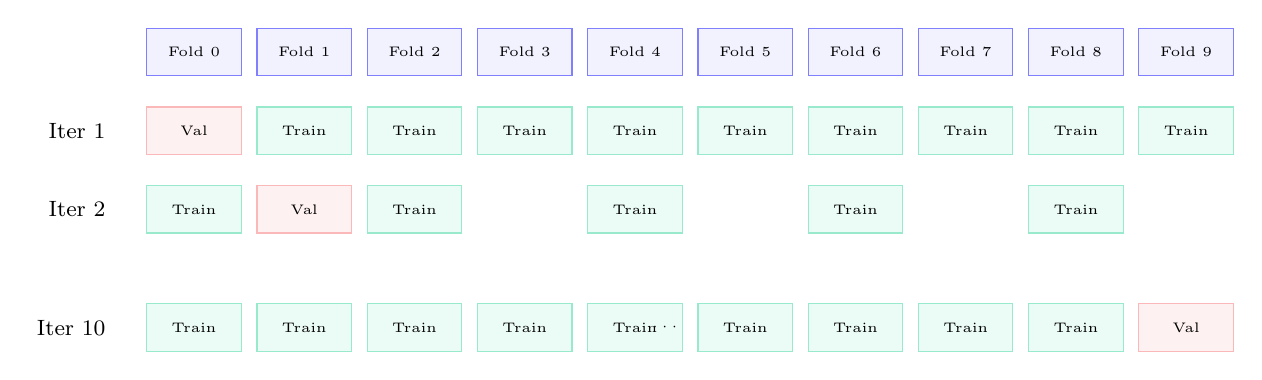
\begin{tikzpicture}[
    node distance=0.8cm,
    fold/.style={rectangle, draw=blue!50, fill=blue!5, minimum width=1.2cm, minimum height=0.6cm, font=\tiny},
    train/.style={rectangle, draw=green!50, fill=green!10, minimum width=1.2cm, minimum height=0.6cm, font=\tiny},
    val/.style={rectangle, draw=red!50, fill=red!10, minimum width=1.2cm, minimum height=0.6cm, font=\tiny},
]
    % Fold labels
    \foreach \i in {0,...,9} {
        \node[fold] at (\i*1.4, 0) {Fold \i};
    }
    % Iteration 1
    \foreach \i in {1,...,9} { \node[train] at (\i*1.4, -1) {Train}; }
    \node[val] at (0, -1) {Val};
    % Iteration 2
    \foreach \i in {0,2,...,9} { \node[train] at (\i*1.4, -2) {Train}; }
    \node[val] at (1.4, -2) {Val};
    % Iteration 10
    \foreach \i in {0,...,8} { \node[train] at (\i*1.4, -3.5) {Train}; }
    \node[val] at (12.6, -3.5) {Val};
    \node[font=\tiny] at (6, -3.5) {$\cdots$};
    % Labels
    \node[font=\footnotesize, anchor=east] at (-1, -1) {Iter 1};
    \node[font=\footnotesize, anchor=east] at (-1, -2) {Iter 2};
    \node[font=\footnotesize, anchor=east] at (-1, -3.5) {Iter 10};
\end{tikzpicture}
\caption{10-fold cross-validation: each fold serves as the validation set exactly once. The final score is the average of all 10 iterations, providing a robust estimate of model performance.}
\label{fig:cv}
\end{figure}

\begin{table}[H]
\centering
\caption{Stratified cross-validation results (10 folds, F1-Score)}
\label{tab:cv_results}
\begin{tabular}{lcc}
\toprule
\textbf{Model} & \textbf{Mean F1} & \textbf{Std Dev ($\pm 2\sigma$)} \\
\midrule
Random Forest & 0.9993 & $\pm$ 0.0003 \\
XGBoost & 0.9994 & $\pm$ 0.0003 \\
\bottomrule
\end{tabular}
\end{table}

The extremely low standard deviation ($\pm 0.0003$) confirms that both models perform consistently across all folds --- there is no overfitting to a particular subset of the data. Note that Isolation Forest, being unsupervised, cannot be evaluated via cross-validation on F1 score (it never sees labels during training).

\section{Understanding the Evaluation Metrics}

Before presenting the numerical results, it is important to define what each metric actually means. In network intrusion detection, different metrics serve different purposes:

\begin{itemize}
    \item \textbf{Accuracy} — The percentage of all predictions that were correct: $\frac{TP + TN}{TP + TN + FP + FN}$. This is the simplest metric but can be misleading if the classes are imbalanced.

    \item \textbf{Precision} — Of all the flows the model flagged as attacks, what percentage actually were attacks: $\frac{TP}{TP + FP}$. \textbf{High precision means few false alarms.}

    \item \textbf{Recall} — Of all the actual attack flows in the data, what percentage did the model catch: $\frac{TP}{TP + FN}$. \textbf{High recall means few missed attacks.}

    \item \textbf{F1-Score} — The harmonic mean of precision and recall: $2 \times \frac{P \times R}{P + R}$. This is the best single-number summary when both false alarms and missed attacks matter.

    \item \textbf{False Positive Rate (FPR)} — What percentage of benign flows were incorrectly flagged as attacks: $\frac{FP}{FP + TN}$. \textbf{Low FPR means the system does not cry wolf.}

    \item \textbf{AUC-ROC} — The area under the ROC curve. A value of 0.5 means the model is no better than random guessing; 1.0 means perfect discrimination at every threshold.
\end{itemize}

\begin{table}[H]
\centering
\caption{Confusion matrix terminology}
\label{tab:cm_terms}
\begin{tabular}{llp{7cm}}
\toprule
\textbf{Term} & \textbf{Meaning} & \textbf{In our context} \\
\midrule
TP (True Positive) & Correctly classified as attack & Port scan correctly detected as port scan \\
TN (True Negative) & Correctly classified as benign & Normal traffic correctly identified as normal \\
FP (False Positive) & Benign incorrectly classified as attack & Normal traffic falsely triggers an alert \\
FN (False Negative) & Attack missed (classified as benign) & Port scan goes undetected \\
\bottomrule
\end{tabular}
\end{table}

\noindent\textbf{Where:} $TP$ = True Positive, $TN$ = True Negative, $FP$ = False Positive, $FN$ = False Negative.

\section{Results and Analysis}

\subsection{Supervised Models: Random Forest and XGBoost}

Both supervised models deliver exceptional performance on the CICIDS2017 test set:

\begin{table}[H]
\centering
\caption{Performance comparison of all three models on the CICIDS2017 test set (57,294 samples)}
\label{tab:results}
\begin{tabular}{lcccccc}
\toprule
\textbf{Model} & \textbf{Accuracy} & \textbf{Precision} & \textbf{Recall} & \textbf{F1-Score} & \textbf{AUC-ROC} & \textbf{FPR} \\
\midrule
Random Forest & 99.911\% & 99.909\% & 99.931\% & 99.920\% & 0.9997 & 0.114\% \\
XGBoost & 99.914\% & 99.909\% & 99.937\% & 99.923\% & 0.9999 & 0.114\% \\
Isolation Forest & 24.627\% & 14.184\% & 7.101\% & 9.464\% & --- & 53.532\% \\
\bottomrule
\end{tabular}
\end{table}

\textbf{What these numbers mean in practice:}
\begin{itemize}
    \item Out of 57,294 test flows (31,786 attacks + 25,508 benign), Random Forest makes only 51 mistakes total: 29 false positives (benign flagged as attack) and 22 false negatives (attacks missed).
    \item XGBoost makes 49 mistakes: 29 false positives and 20 false negatives.
    \item The 0.114\% FPR means that out of 1,000 benign flows, the system incorrectly raises an alert for approximately 1 --- an acceptable rate for a production environment.
\end{itemize}

\begin{figure}[H]
\centering
\begin{subfigure}[b]{0.48\textwidth}
\includegraphics[width=\textwidth]{confusion_matrix_random_forest.png}\caption{Random Forest}\end{subfigure}\hfill
\begin{subfigure}[b]{0.48\textwidth}
\includegraphics[width=\textwidth]{confusion_matrix_xgboost.png}\caption{XGBoost}\end{subfigure}
\caption{Confusion matrices for the supervised models. Both models make very few errors: the vast majority of predictions fall on the diagonal (correct classifications).}
\label{fig:confusion_matrices}
\end{figure}

\begin{figure}[H]
\centering
\begin{subfigure}[b]{0.48\textwidth}
\includegraphics[width=\textwidth]{roc_random_forest.png}\caption{Random Forest}\end{subfigure}\hfill
\begin{subfigure}[b]{0.48\textwidth}
\includegraphics[width=\textwidth]{roc_xgboost.png}\caption{XGBoost}\end{subfigure}
\caption{ROC curves for the supervised models. Both achieve AUC $> 0.999$, indicating near-perfect discrimination between BENIGN and PortScan traffic at every possible classification threshold.}
\label{fig:roc_curves}
\end{figure}

\subsection{Success Criteria Verification}

The project's final plan defines three quantitative thresholds. Both supervised models not only meet these criteria --- they vastly exceed them:

\begin{table}[H]
\centering
\caption{Verification of project success criteria}
\label{tab:success}
\begin{tabular}{lccccc}
\toprule
\textbf{Criterion} & \textbf{Threshold} & \textbf{RF} & \textbf{Status} & \textbf{XGBoost} & \textbf{Status} \\
\midrule
F1-Score & $\geq$ 88\% & 99.920\% & \textbf{PASS} & 99.923\% & \textbf{PASS} \\
Accuracy & $\geq$ 90\% & 99.911\% & \textbf{PASS} & 99.914\% & \textbf{PASS} \\
FPR & $<$ 6\% & 0.114\% & \textbf{PASS} & 0.114\% & \textbf{PASS} \\
\bottomrule
\end{tabular}
\end{table}

\subsection{Analysis of Isolation Forest's Failure}

Isolation Forest performs very poorly on the CICIDS2017 dataset: with an F1-Score of only 9.46\% and an FPR of 53.53\%, it is essentially unusable for this dataset. However, this result is expected and does not indicate a flaw in the choice of algorithm --- it reveals a fundamental property of the dataset.

\subsubsection{The Majority Anomaly Paradox}

Isolation Forest is designed to detect anomalies -- data points that are \textit{few and different} from the rest of the dataset. The algorithm works by randomly partitioning the feature space: points that can be isolated with few partitions (short average path length in the isolation tree) are considered anomalies.

This assumption works well when anomalies represent a small fraction of the data (typically $<$ 5\%). However, in our CICIDS2017 dataset, the PortScan class constitutes \textbf{55.48\%} of the data -- it is the \textbf{majority} class, not a minority:

\begin{figure}[H]
\centering
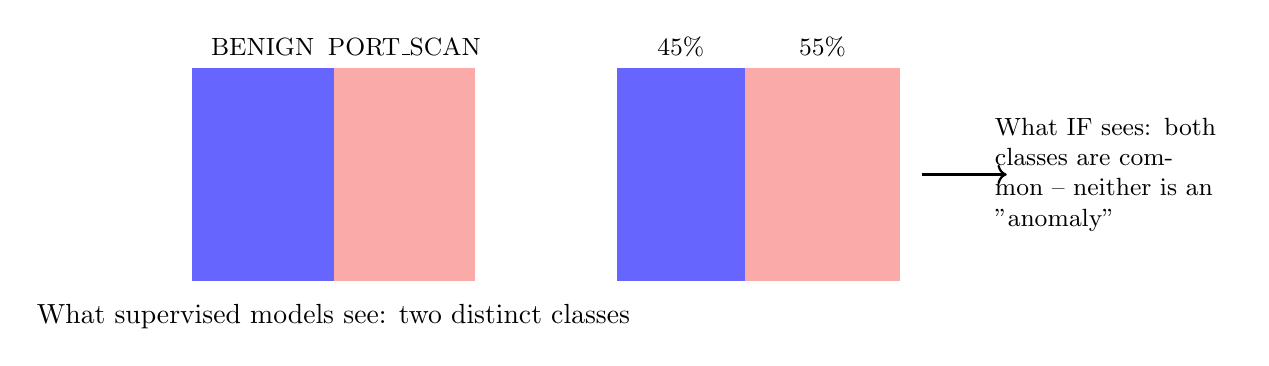
\begin{tikzpicture}[scale=0.9]
    % Bar for RF/XGB
    \fill[blue!60] (0,0) rectangle (2, 3);
    \fill[red!60] (2,0) rectangle (4, 3);
    \node[font=\small] at (1, 3.3) {BENIGN};
    \node[font=\small] at (3, 3.3) {PORT\_SCAN};
    \node[font=\normalsize] at (2, -0.5) {What supervised models see: two distinct classes};

    % Bar for IF
    \fill[blue!60] (6,0) rectangle (7.8, 3);
    \fill[red!60] (7.8,0) rectangle (10, 3);
    \node[font=\small] at (6.9, 3.3) {45\%};
    \node[font=\small] at (8.9, 3.3) {55\%};
    \draw[->, thick] (10.3, 1.5) -- (11.5, 1.5);
    \node[font=\small, text width=3cm] at (13, 1.5) {What IF sees: both classes are common -- neither is an "anomaly"};
\end{tikzpicture}
\caption{The majority anomaly paradox: when the "anomaly" (PortScan) is actually the majority class, Isolation Forest cannot isolate it as being \textit{few and different}.}
\label{fig:majority_paradox}
\end{figure}

Because the algorithm is trained on the complete dataset (BENIGN + PortScan), it sees both classes as \textit{normal} -- neither is anomalous enough to be separated from the other. The result is a model that essentially guesses at random, with a heavy bias towards the majority class.

\subsubsection{Why We Still Keep Isolation Forest}

Despite its poor performance on CICIDS2017, Isolation Forest remains part of the AEGIS architecture for two reasons:

\begin{enumerate}
    \item \textbf{Correct deployment strategy:} In production, Isolation Forest should be trained exclusively on verified \textbf{BENIGN} traffic to establish a clean baseline of normal network behavior. When trained this way (semi-supervised), it can effectively detect anything deviating from normal -- including never-before-seen attack patterns.

    \item \textbf{Complementary detection:} Supervised models (RF, XGBoost) detect \textit{known} attack patterns they were trained on. Isolation Forest, trained on benign-only data, can detect \textit{unknown} patterns -- low-and-slow scans, custom scanners, zero-day reconnaissance techniques. The two approaches complement each other.
\end{enumerate}

\begin{figure}[H]
\centering

\includegraphics[width=0.5\textwidth]{confusion_matrix_isolation_forest.png}
\caption{Confusion matrix for Isolation Forest on CICIDS2017. The high number of false positives (13,655 benign flows flagged as attacks) and false negatives (29,529 attacks missed) confirms that the unsupervised approach fails when trained on the full imbalanced dataset.}
\label{fig:iso_cm}
\end{figure}

\section{Conclusion}

This chapter presented the training and evaluation of the three models that form the core of the AEGIS detection pipeline. The results are clear:

\begin{enumerate}
    \item \textbf{Supervised models dominate on this problem.} Random Forest and XGBoost achieve F1-Scores exceeding 99.92\%, with FPRs below 0.12\%. Both models far exceed the project's success criteria (F1 $\geq$ 88\%, Accuracy $\geq$ 90\%, FPR $<$ 6\%). The 10-fold cross-validation confirms these results are stable and reproducible.

    \item \textbf{Isolation Forest fails on CICIDS2017 for a predictable reason.} The majority anomaly paradox -- PortScan being 55\% of the data -- prevents the unsupervised algorithm from usefully separating the classes. This is not a flaw in the algorithm but a mismatch between the training strategy (full dataset, unsupervised) and what the algorithm requires (benign-only, semi-supervised). In a production environment with benign-only training, the model would regain its relevance.

    \item \textbf{The feature set is sufficient.} With only 11 features, both supervised models achieve near-perfect classification. This validates the feature selection done in Chapter~4 and suggests that the 9 CICIDS2017 features carry strong discriminative signal for port scan detection. The 2 placeholder features (shadow node interaction, MTD port delta) will provide additional signal when integrated with the real-time defense subsystems (Chapter~7).
\end{enumerate}

The trained models are saved in \texttt{models/saved/} and are ready for integration with the capture layer (Chapter~6), the defense subsystem (Chapter~7), and the dashboard (Chapter~8).


% ============================================
% CHAPTER 6: Capture and Network Lab
% ============================================
\input{chapters/ch06_capture}

% ============================================
% CHAPTER 7: Defense and Deception Subsystem
% ============================================
\input{chapters/ch07_defense}

% ============================================
% CHAPTER 8: Integration and Deployment
% ============================================
\input{chapters/ch08_integration}

% ============================================
% CHAPTER 9: Test and Validation
% ============================================
\input{chapters/ch09_test_validation}

% ============================================
% CHAPTER 10: General Conclusion
% ============================================
\input{chapters/ch10_conclusion}

% --- Bibliography ---
\bibliographystyle{plain}
\bibliography{references}

\end{document}
